\documentclass[11pt,a4paper]{book}
\usepackage[italian]{babel}
\usepackage[T1]{fontenc}
\usepackage[utf8]{inputenc}
\usepackage{lmodern}
\usepackage{geometry}
\geometry{margin=2.5cm}
\usepackage{graphicx}
\usepackage{xcolor}
\usepackage{listings}
\usepackage{amsmath}
\usepackage{booktabs}
\usepackage{hyperref}
\usepackage{float}
\lstdefinestyle{python}{language=Python,basicstyle=\ttfamily\small,keywordstyle=\color{blue!70!black},commentstyle=\color{green!40!black},stringstyle=\color{red!60!black},numbers=left,numberstyle=\tiny,frame=single,breaklines=true,showstringspaces=false}
\lstset{style=python}
\title{Costruire figure scientifiche con Python\\Un percorso graduale con NumPy e Matplotlib}
\author{Giuseppe Mandaglio}
\date{}
\begin{document}
\maketitle
\tableofcontents

\chapter{Introduzione}
Questo documento sviluppa passo dopo passo una figura scientifica in Python. Si parte da un grafico minimo e si aggiungono marker, legenda, etichette, più serie di dati, salvataggio su file, barre di errore e personalizzazione grafica. I dati vengono letti con \texttt{numpy.loadtxt}, mentre la rappresentazione grafica è affidata a \texttt{matplotlib.pyplot}.

\section{Struttura dei file di dati}
Nel file \texttt{datios.txt} le colonne rappresentano $x$, $y$, $\sigma_x$ e $\sigma_y$. Nel file allegato \texttt{Kter.txt} sono invece presenti $x$, $y_1$ e $y_2$. Gli script originali indicano \texttt{Kter2.dat}; nel materiale di questo documento il nome è stato uniformato a \texttt{Kter.txt}, che è il file effettivamente disponibile.

\chapter{Dal grafico minimo alla figura completa}
\section{Il grafico più semplice: plot\_bad.py}
\lstinputlisting{plot_bad.py}
\texttt{np.loadtxt} legge l'intera tabella. Le espressioni \texttt{dati[:,0]} e \texttt{dati[:,1]} selezionano rispettivamente la prima e la seconda colonna. Senza uno stile esplicito, \texttt{plot} collega i punti con una linea.
\begin{figure}[H]\centering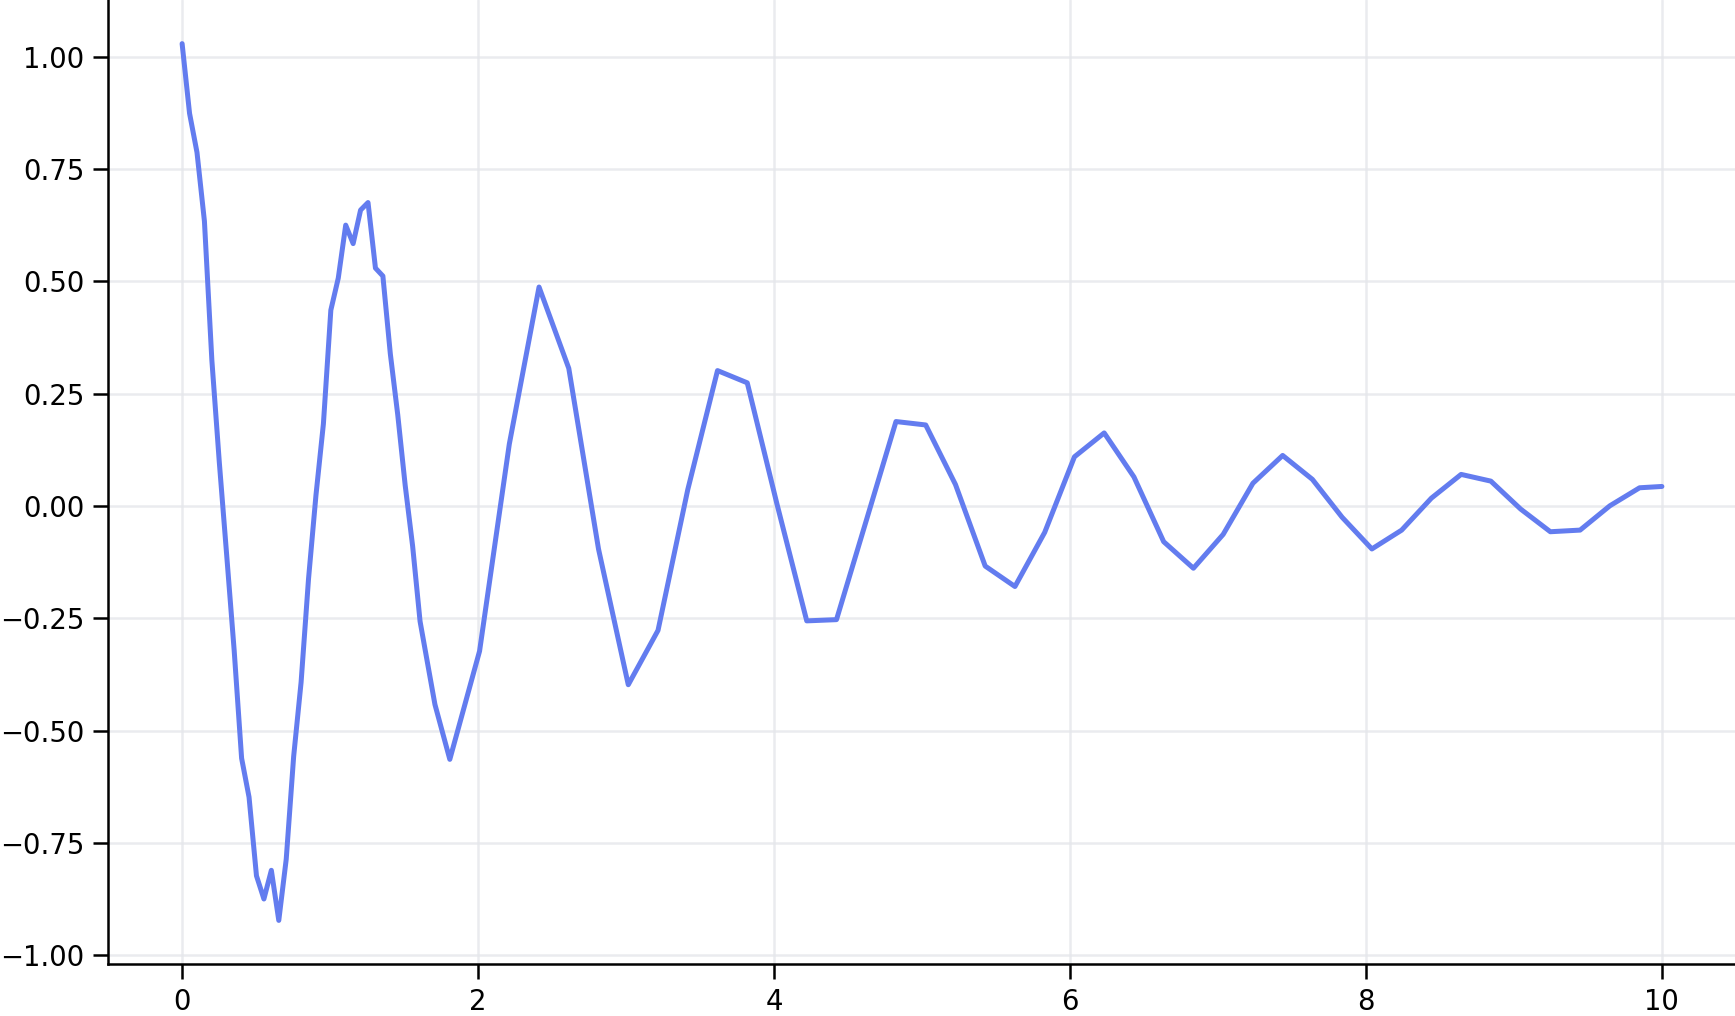
\includegraphics[width=.78\textwidth]{fig_plot_bad.png}\caption{Risultato di \texttt{plot\_bad.py}.}\end{figure}

\section{Visualizzare punti separati: plot\_bad2.py}
\lstinputlisting{plot_bad2.py}
La stringa di formato \texttt{"o"} richiede marker circolari e, non specificando una linea, evita di collegare i punti.
\begin{figure}[H]\centering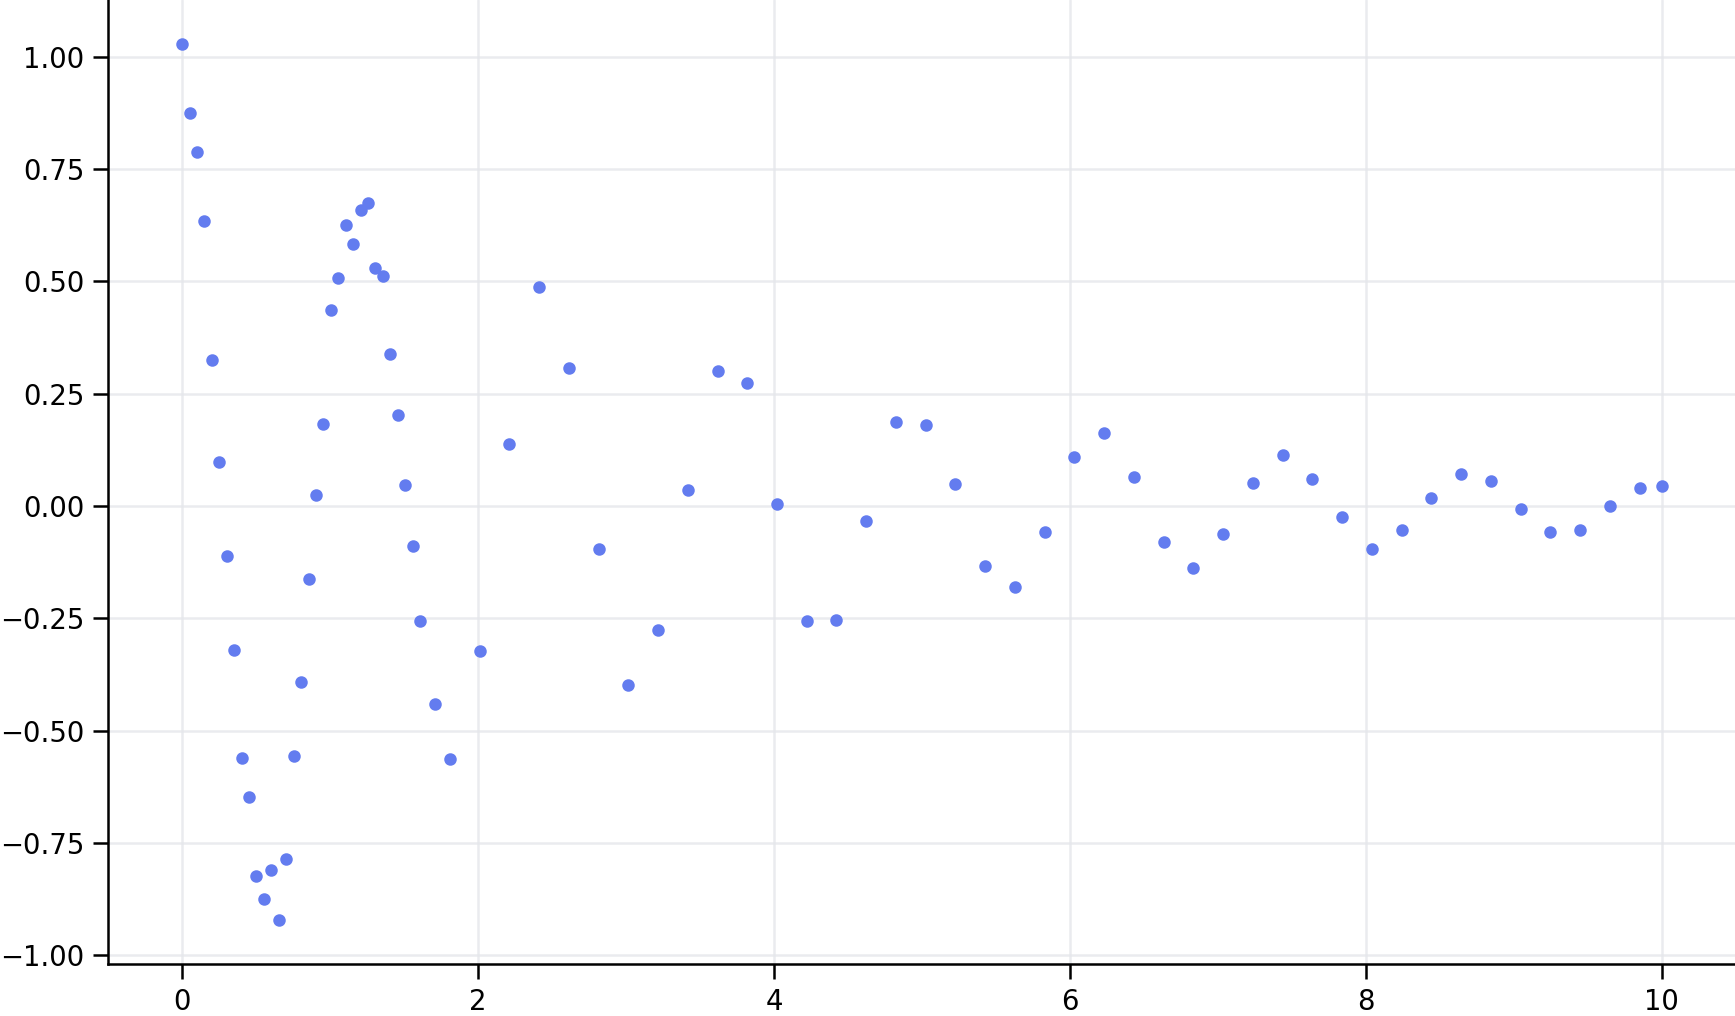
\includegraphics[width=.78\textwidth]{fig_plot_bad2.png}\caption{Dati rappresentati con marker circolari.}\end{figure}

\section{Etichetta e legenda: plot\_bad3.py}
\lstinputlisting{plot_bad3.py}
Il marker \texttt{"\string^"} produce triangoli. L'argomento \texttt{label} assegna un nome alla serie, mentre \texttt{legend()} crea la legenda.
\begin{figure}[H]\centering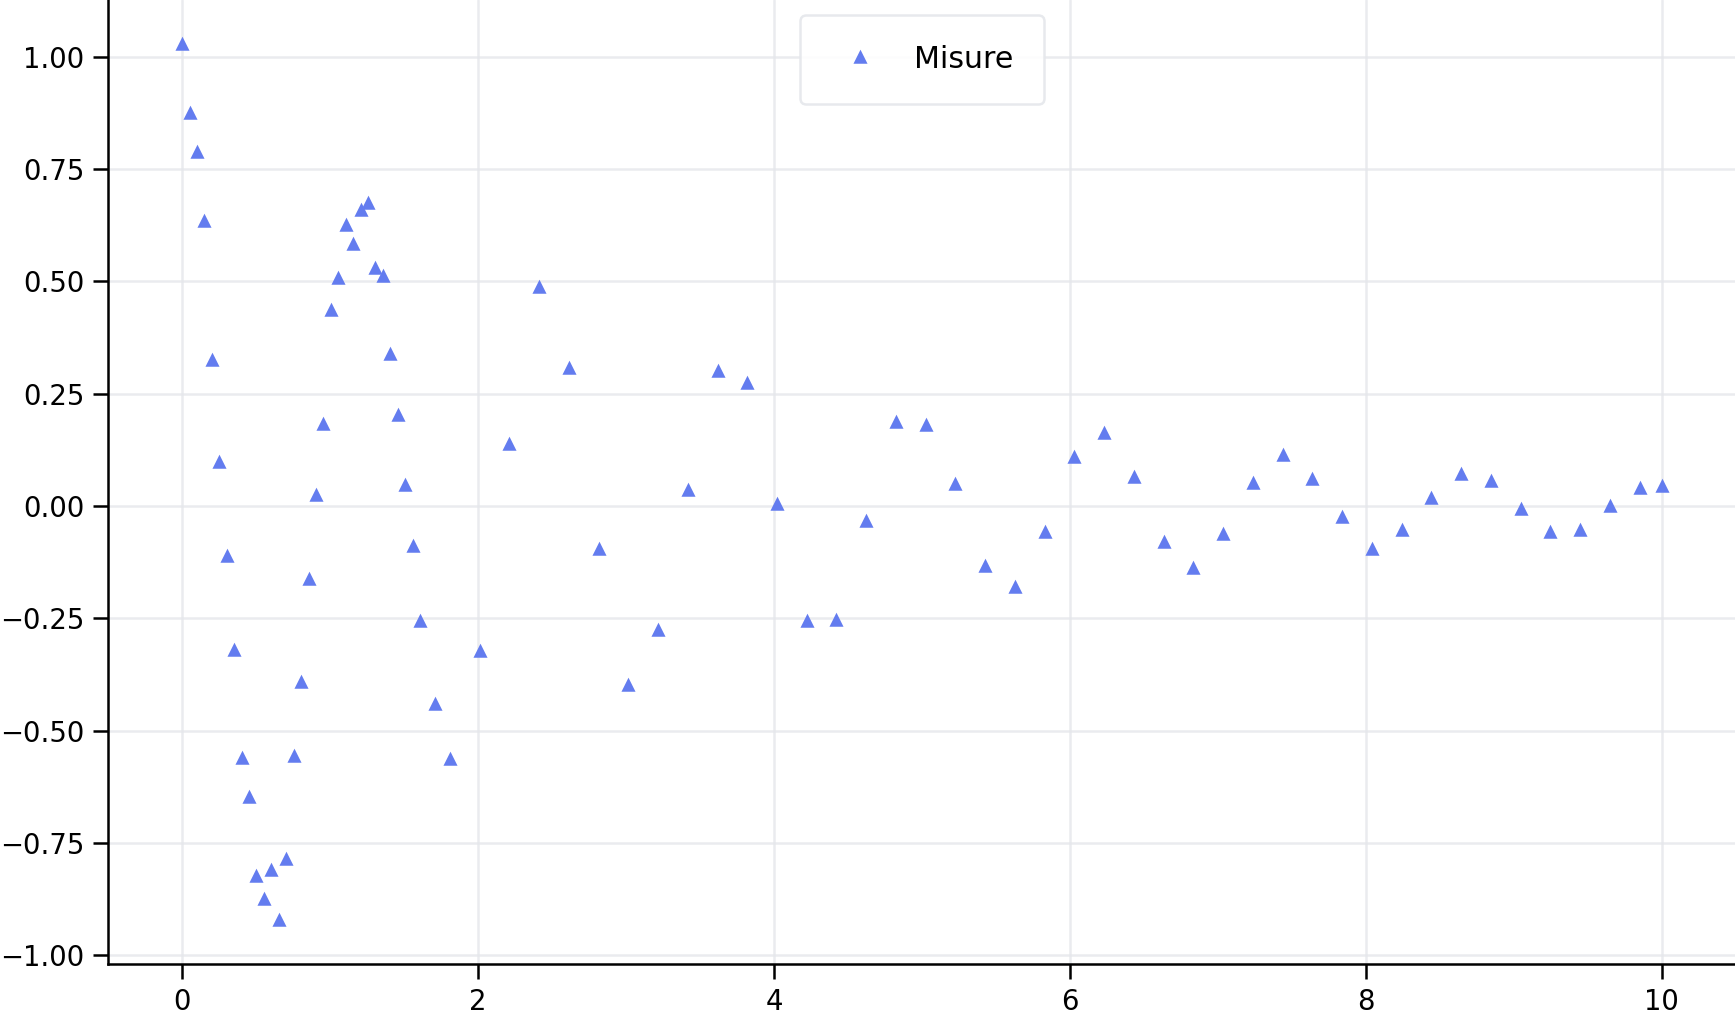
\includegraphics[width=.78\textwidth]{fig_plot_bad3.png}\caption{Marker triangolari e legenda.}\end{figure}

\section{Nomi e unità sugli assi: plot\_bad4.py}
\lstinputlisting{plot_bad4.py}
Le funzioni \texttt{xlabel} e \texttt{ylabel} descrivono le grandezze riportate sugli assi. In una figura scientifica è buona pratica indicare sempre anche le unità di misura.
\begin{figure}[H]\centering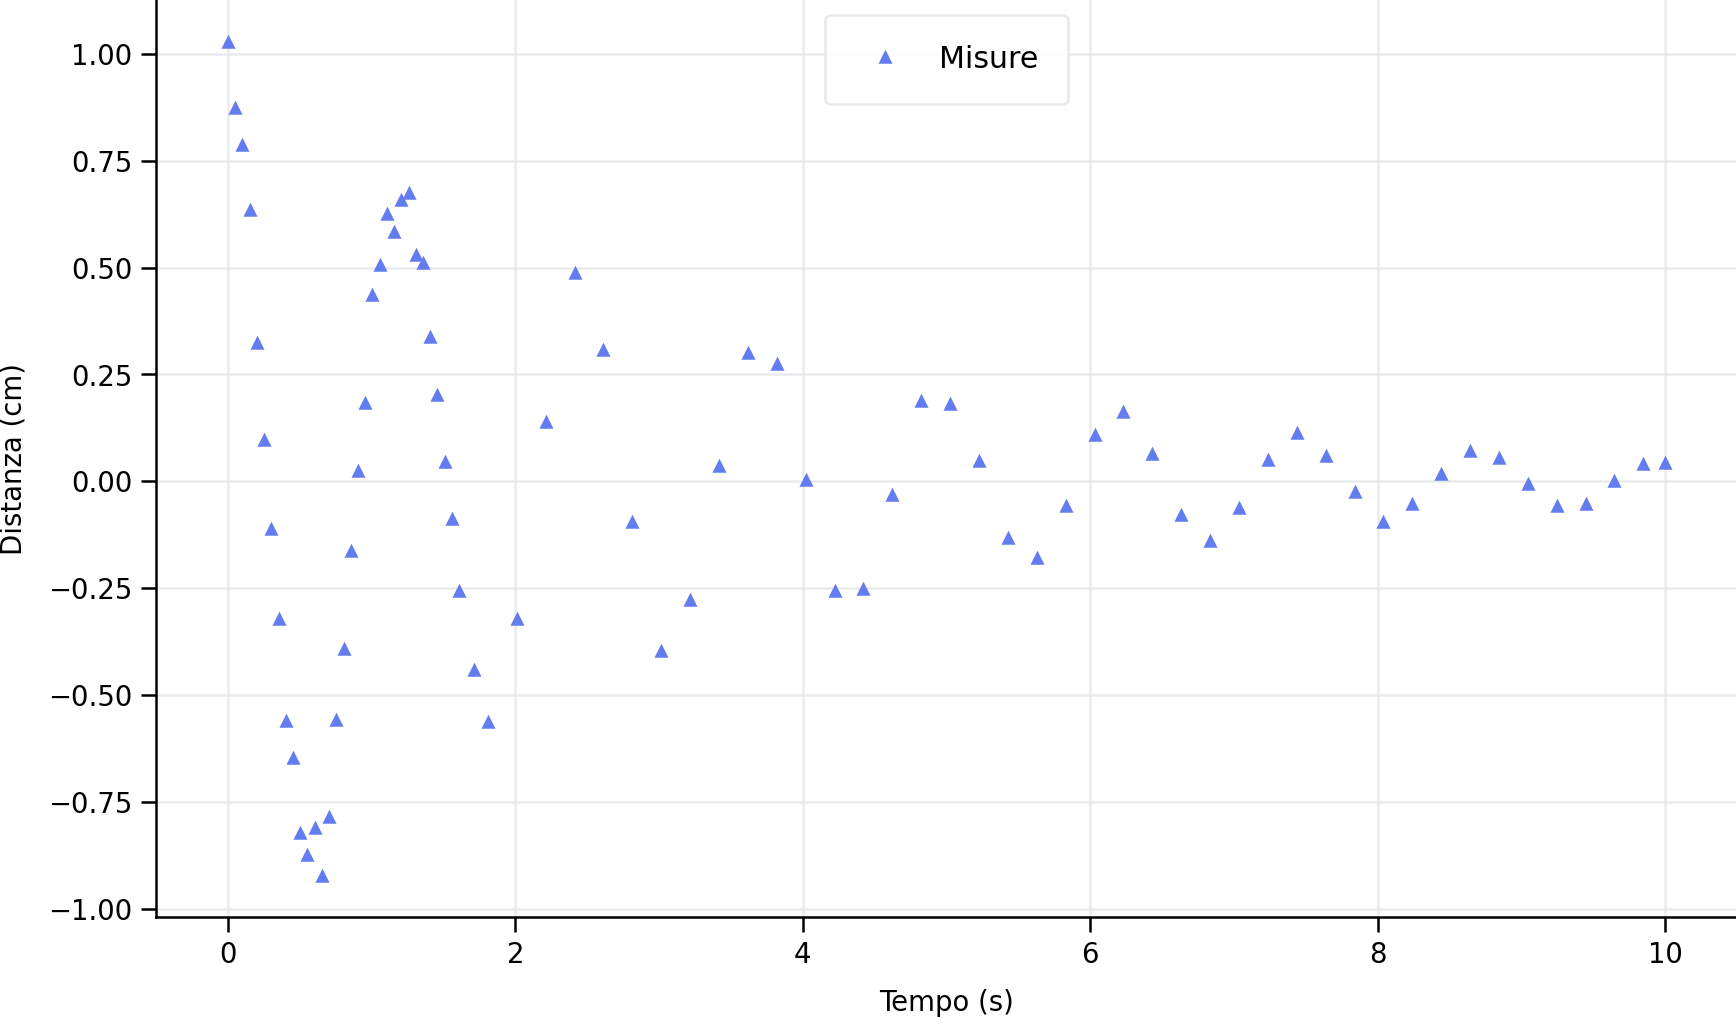
\includegraphics[width=.78\textwidth]{fig_plot_bad4.png}\caption{Figura con etichette degli assi.}\end{figure}

\section{Due misure nella stessa figura: plot\_bad5.py}
\lstinputlisting{plot_bad5.py}
La terza colonna introduce una seconda serie. Due chiamate a \texttt{plot} disegnano le serie nello stesso sistema di assi; marker e label differenti consentono di distinguerle.
\begin{figure}[H]\centering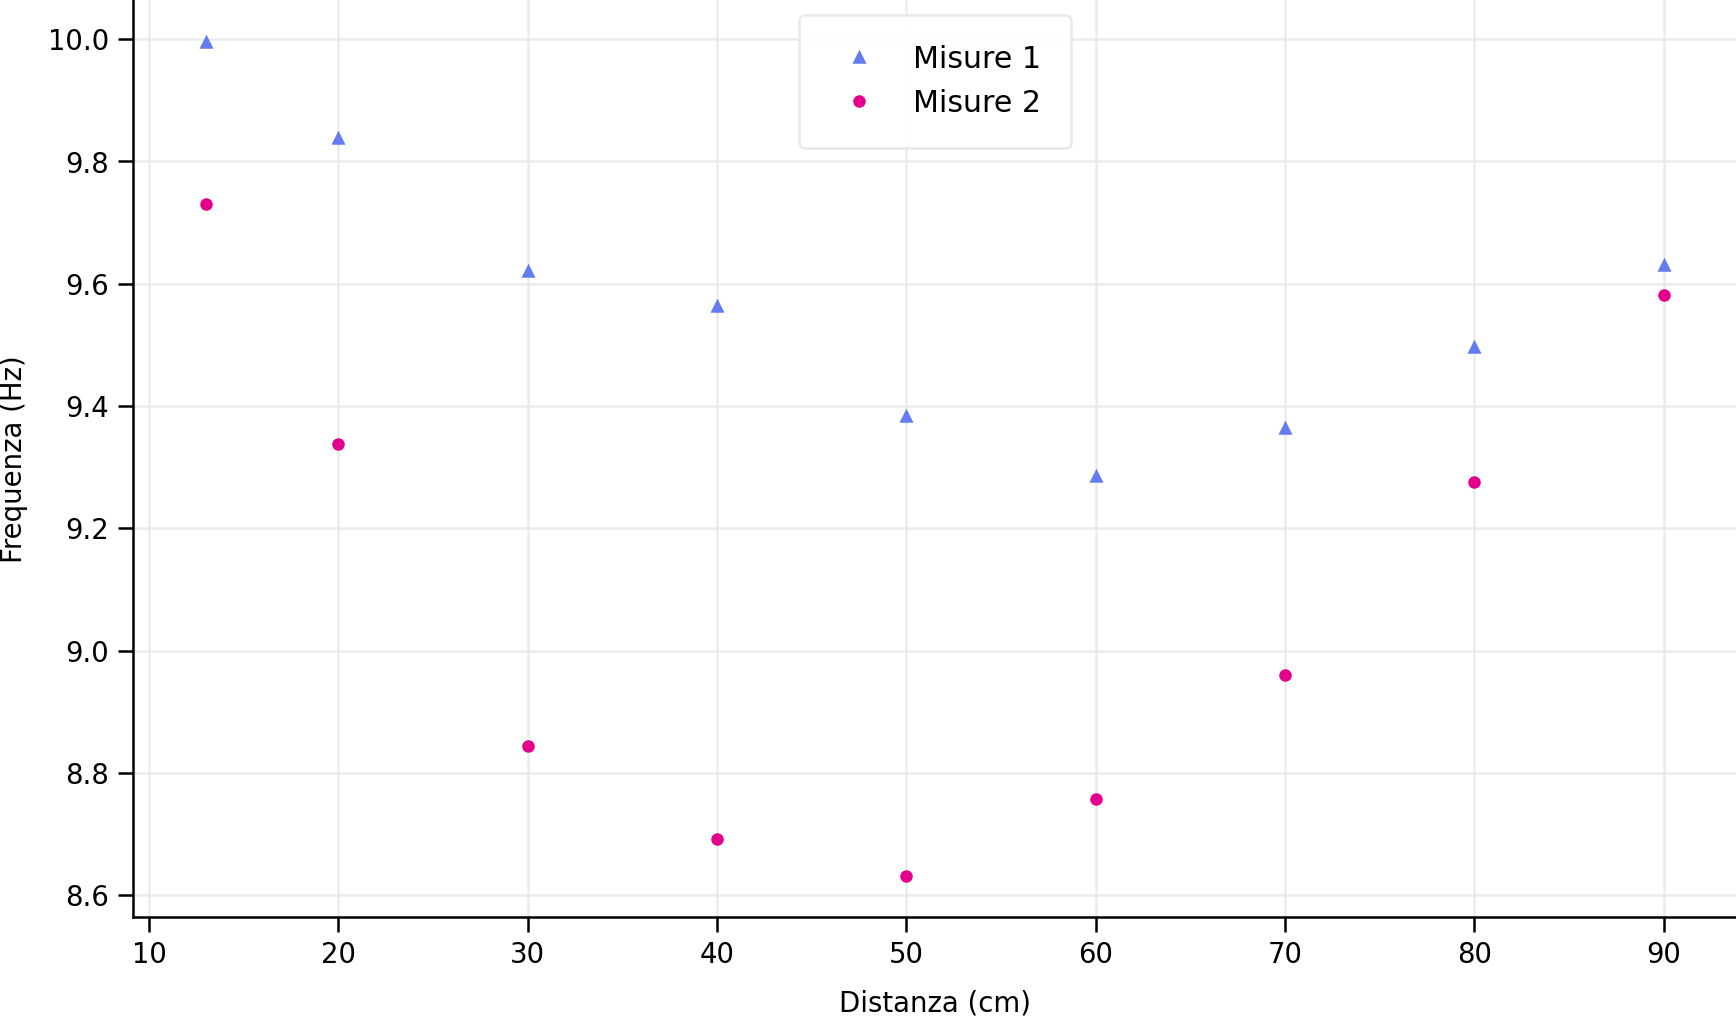
\includegraphics[width=.78\textwidth]{fig_plot_bad5.png}\caption{Confronto tra due serie di misure.}\end{figure}

\section{Lettura compatta e salvataggio: plot\_bad6.py}
\lstinputlisting{plot_bad6.py}
Con \texttt{unpack=True}, ogni colonna viene restituita come array separato. Il salvataggio in PDF mantiene una grafica vettoriale; nel PNG il parametro \texttt{dpi=300} imposta una risoluzione adatta alla stampa. È preferibile salvare prima di \texttt{show()}, perché alcuni backend possono chiudere o svuotare la figura dopo la visualizzazione.
\begin{figure}[H]\centering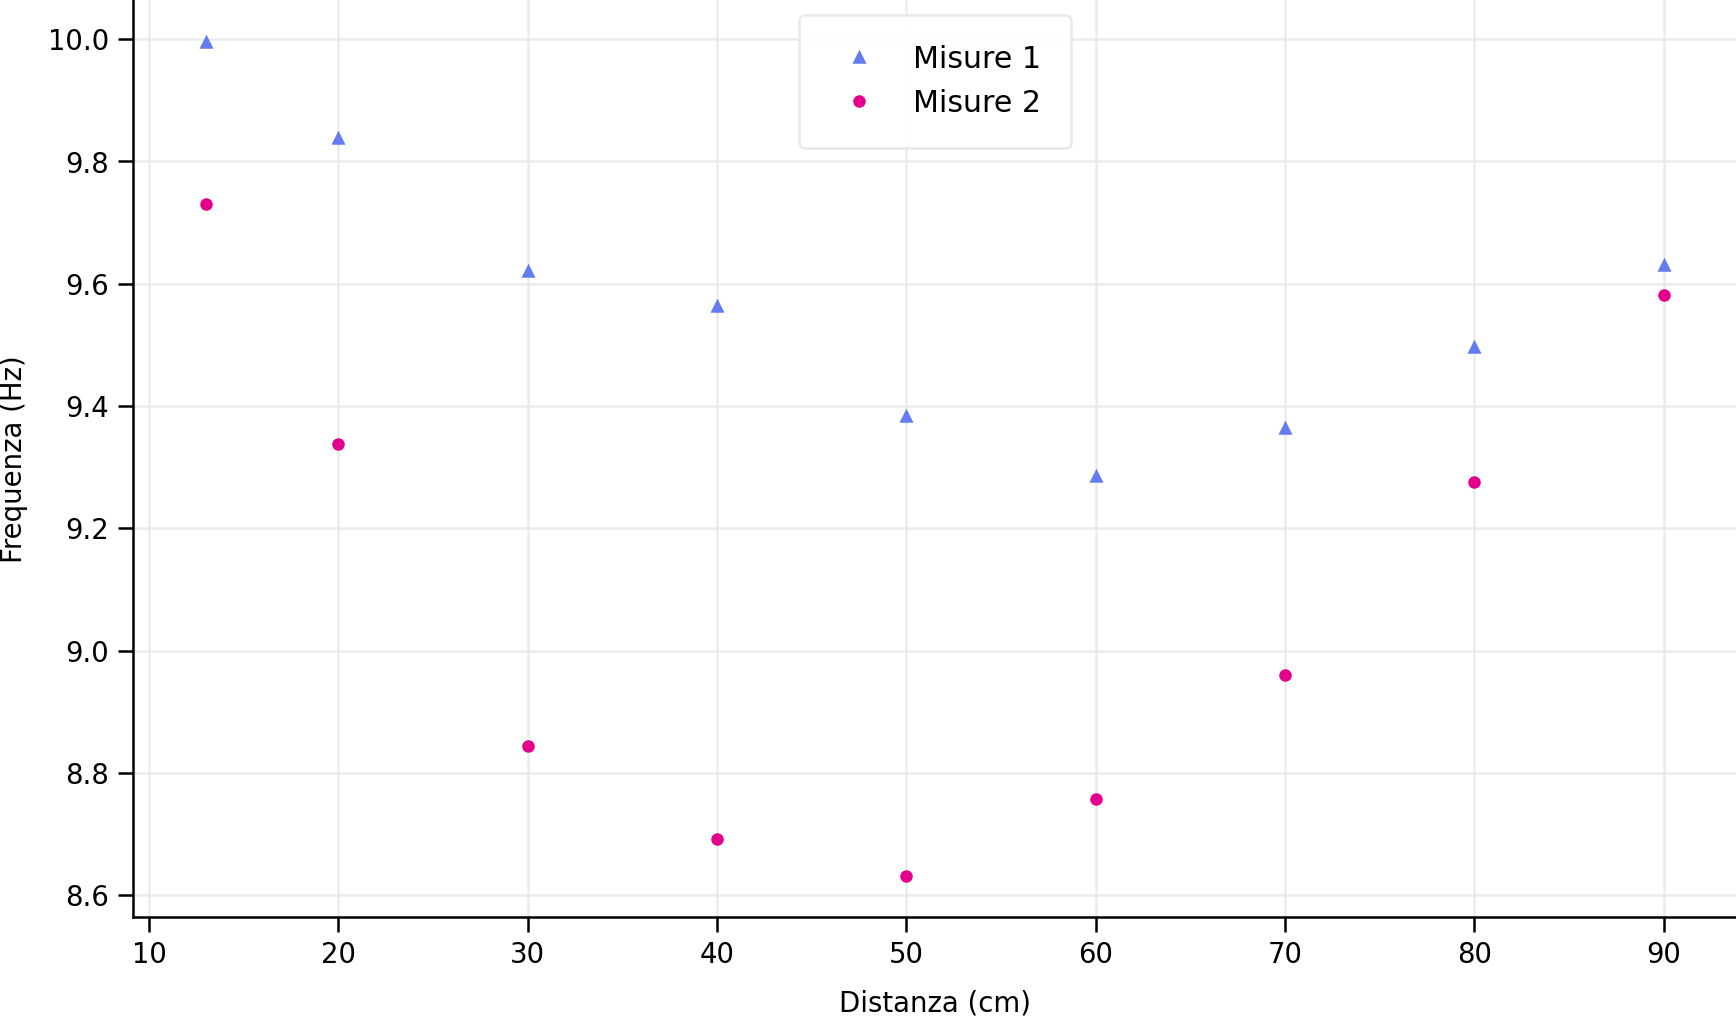
\includegraphics[width=.78\textwidth]{fig_plot_bad6.png}\caption{Figura a due serie salvabile in PDF e PNG.}\end{figure}

\section{Versione rifinita: plottos2.py}
La versione più completa usa l'interfaccia orientata agli oggetti di Matplotlib:
\begin{lstlisting}
fig, ax = plt.subplots(figsize=(8, 6))
ax.errorbar(x, y, xerr=xerr, yerr=yerr,
            fmt="o", color="blue", ecolor="gray",
            elinewidth=1, capsize=3, markersize=5,
            label="Misura")
\end{lstlisting}
\texttt{fig} rappresenta l'intera figura, mentre \texttt{ax} è il sistema di assi su cui si opera. \texttt{errorbar} accetta gli errori orizzontali e verticali. \texttt{fmt} controlla il marker, \texttt{ecolor} il colore delle barre, \texttt{elinewidth} il loro spessore e \texttt{capsize} la lunghezza dei terminali.

Le etichette sono personalizzate con \texttt{ax.set\_xlabel} e \texttt{ax.set\_ylabel}. \texttt{tick\_params} controlla dimensione, spessore e lunghezza dei tick. \texttt{MultipleLocator} stabilisce il passo delle divisioni principali, mentre \texttt{AutoMinorLocator(5)} suddivide ogni intervallo principale in cinque parti. Gli \textit{spines} sono i quattro bordi dell'area del grafico. Infine, \texttt{tight\_layout} riduce il rischio che etichette e numeri vengano tagliati.
\begin{figure}[H]\centering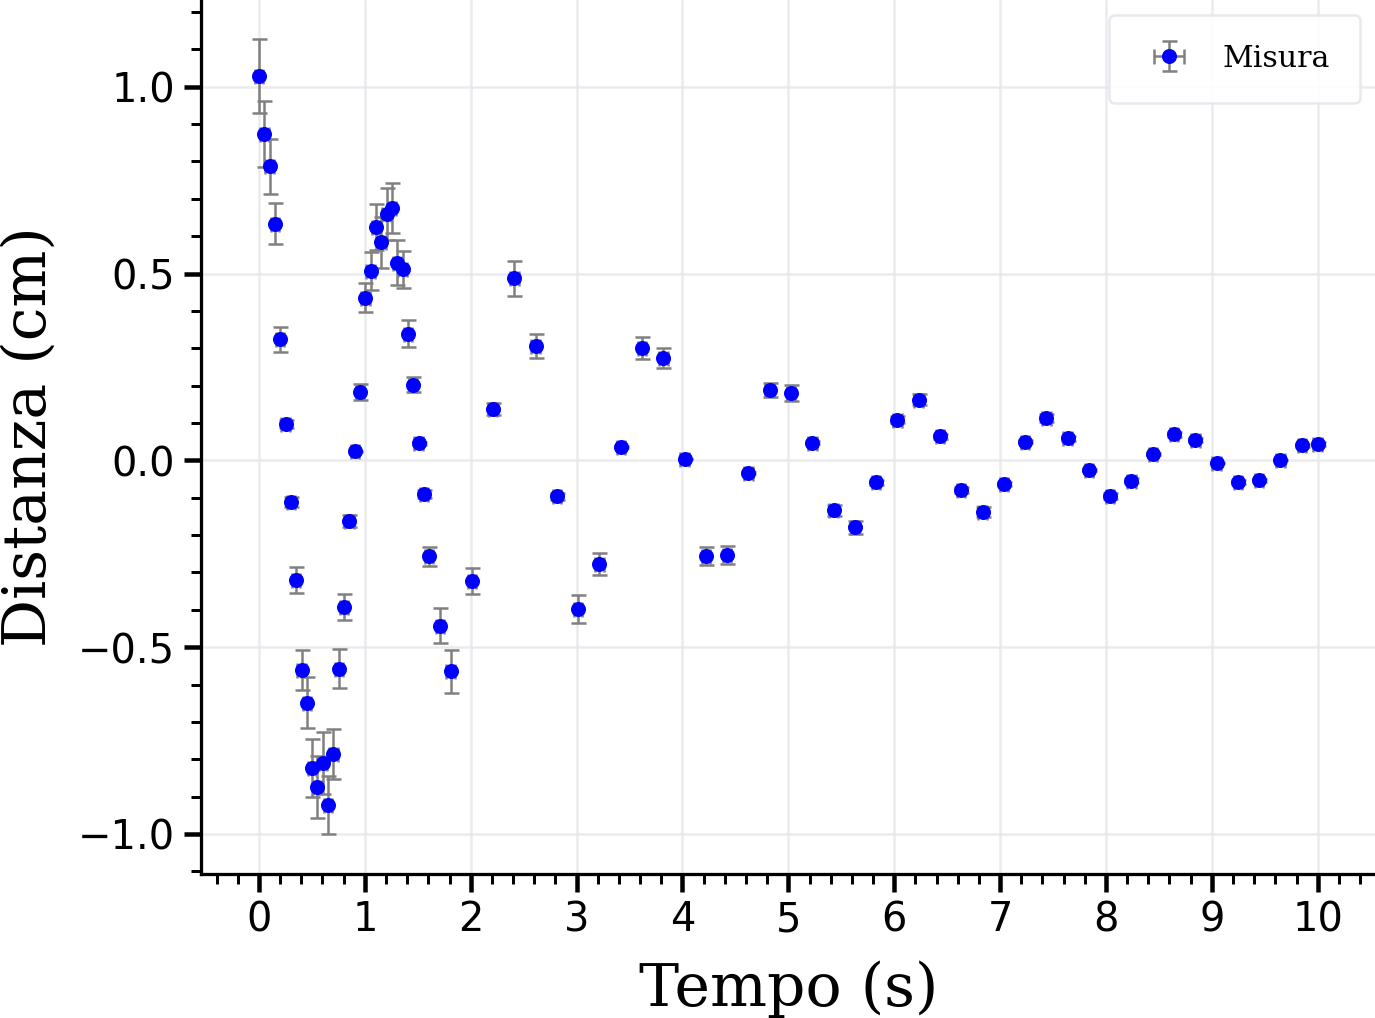
\includegraphics[width=.9\textwidth]{fig_plottos2.png}\caption{Versione rifinita con barre di errore, tick principali e secondari e stile personalizzato.}\end{figure}

\chapter{Fit parabolici con SciPy e NumPy}
\section{Il modello}
Gli script assumono una parabola
\[f(x;a,b,c)=ax^2+bx+c.\]
Il fit determina i parametri che minimizzano la somma dei quadrati dei residui. Se non si forniscono incertezze, ogni punto contribuisce con lo stesso peso.

\section{Fit con scipy.optimize.curve\_fit}
\begin{lstlisting}
from scipy.optimize import curve_fit

def parabola(x, a, b, c):
    return a*x**2 + b*x + c

popt1, pcov1 = curve_fit(parabola, x, y1)
perr1 = np.sqrt(np.diag(pcov1))
\end{lstlisting}
\texttt{curve\_fit} accetta una funzione Python esplicita ed è quindi adatto anche a modelli non polinomiali. \texttt{popt1} contiene i parametri ottimali; \texttt{pcov1} è la matrice di covarianza stimata. Le incertezze standard si ricavano dalla radice quadrata degli elementi diagonali.

Per dati con errori $\sigma_y$ noti, una forma più completa è:
\begin{lstlisting}
popt, pcov = curve_fit(parabola, x, y,
                       sigma=yerr,
                       absolute_sigma=True)
\end{lstlisting}
In questo caso si effettua un fit pesato e \texttt{absolute\_sigma=True} interpreta gli errori come incertezze assolute.
\begin{figure}[H]\centering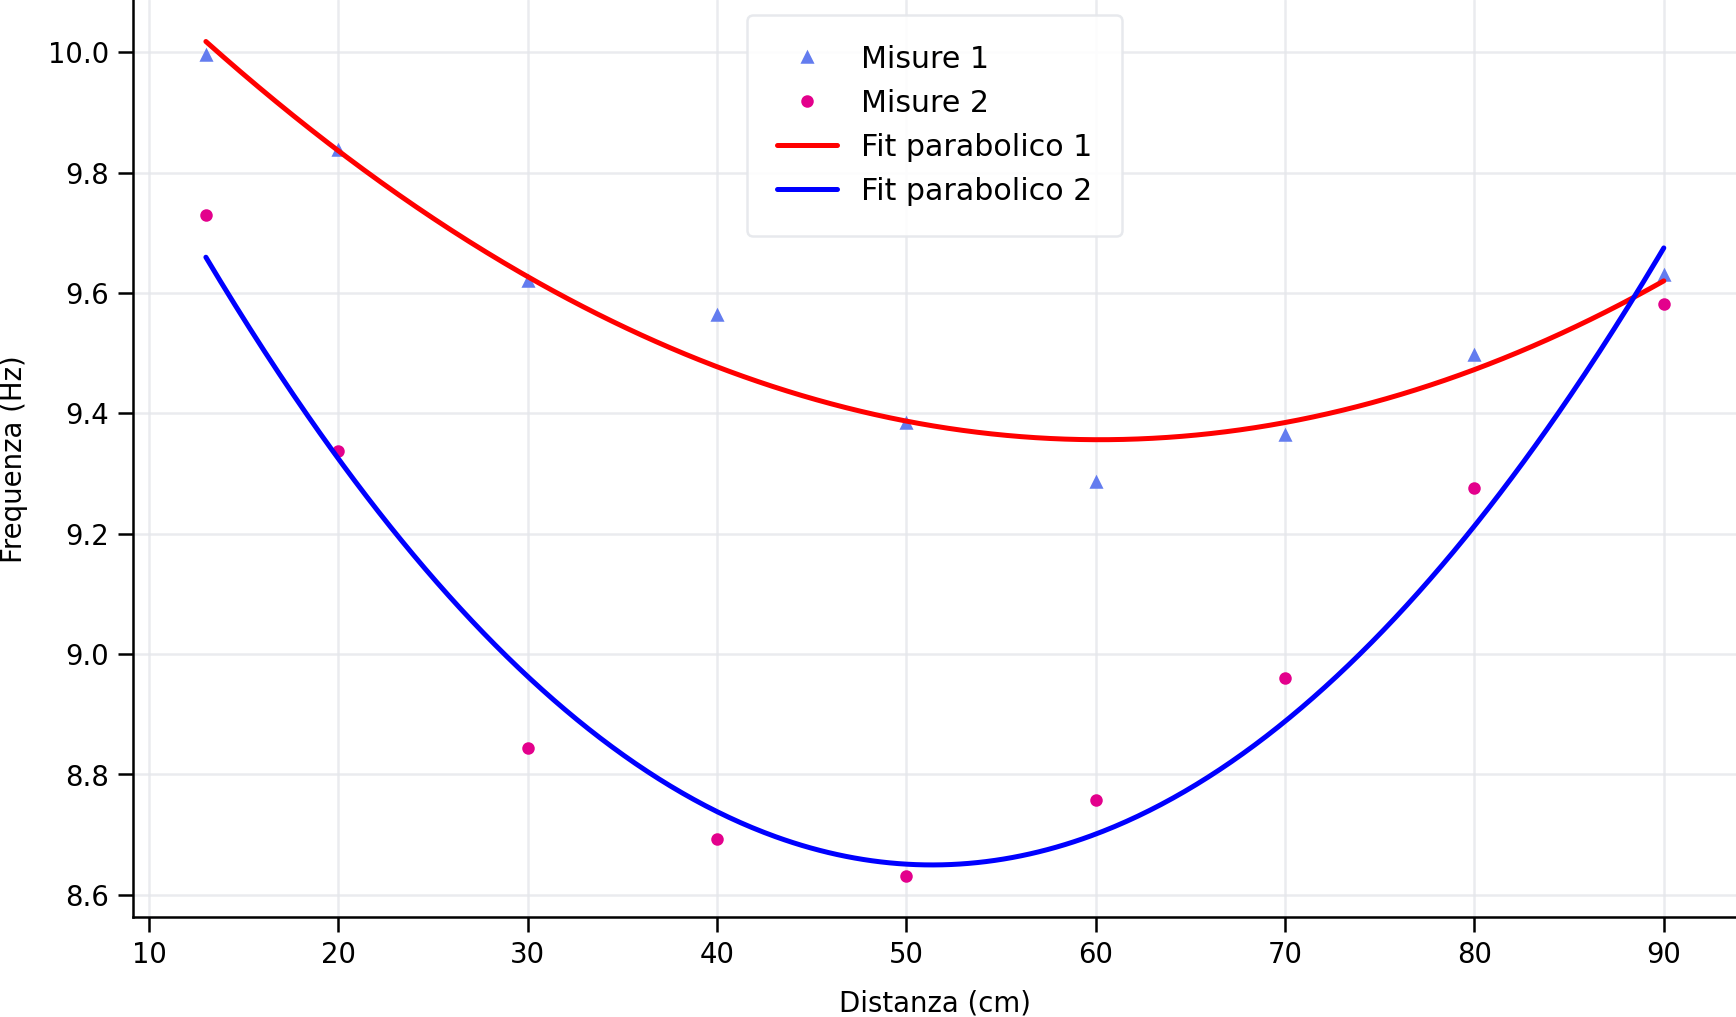
\includegraphics[width=.82\textwidth]{fig_fit_scipy.png}\caption{Fit delle due serie con un modello parabolico.}\end{figure}

\section{Fit con numpy.polyfit}
\begin{lstlisting}
p1 = np.polyfit(x, y1, 2)
yfit1 = np.polyval(p1, xfit)
\end{lstlisting}
Il grado 2 richiede un polinomio quadratico. I coefficienti sono restituiti nell'ordine $[a,b,c]$. \texttt{polyval} valuta il polinomio nei punti della griglia fitta \texttt{xfit}.

\section{Matrice di covarianza e stampa dei risultati}
\begin{lstlisting}
p1, cov1 = np.polyfit(x, y1, 2, cov=True)
err1 = np.sqrt(np.diag(cov1))
print(f"a = {p1[0]:.5g} +/- {err1[0]:.2g}")
\end{lstlisting}
Con \texttt{cov=True}, \texttt{polyfit} restituisce anche la matrice di covarianza. La sintassi della f-string applica cinque cifre significative al valore e due all'errore. Le parentesi quadre devono rimanere all'interno dell'espressione, senza backslash.

Per un fit pesato con \texttt{polyfit}, i pesi sono proporzionali a $1/\sigma_y$:
\begin{lstlisting}
p, cov = np.polyfit(x, y, 2, w=1/yerr, cov=True)
\end{lstlisting}
\begin{figure}[H]\centering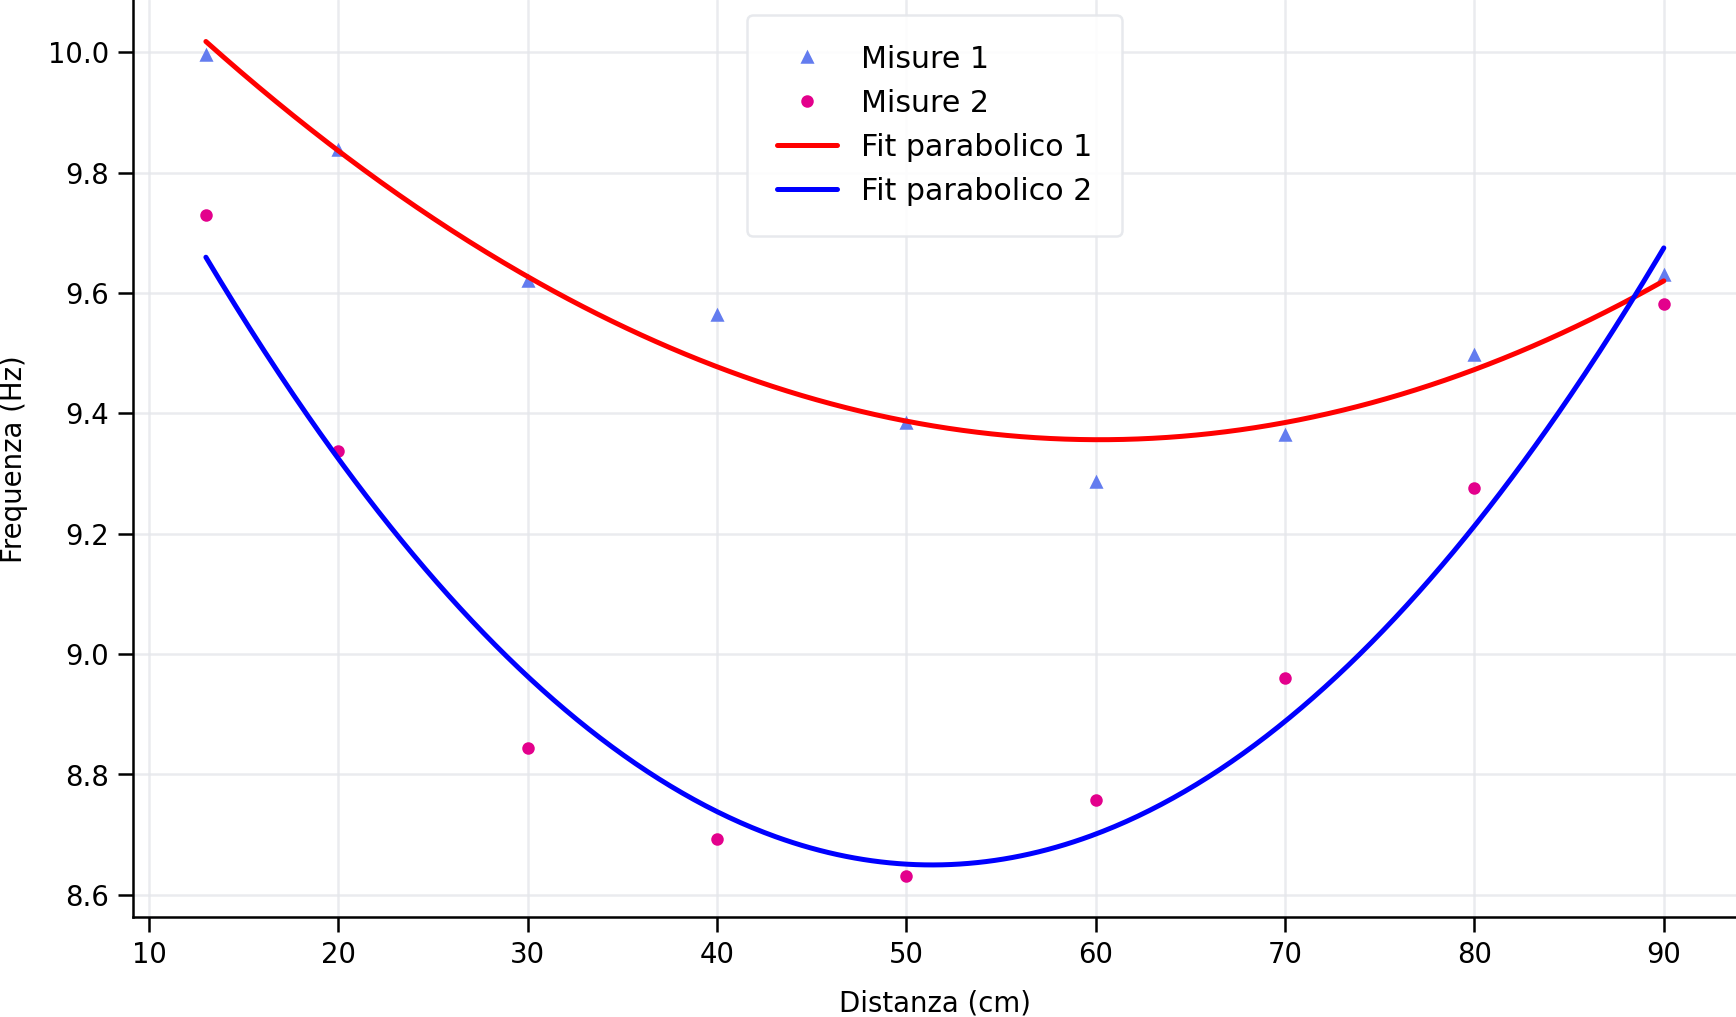
\includegraphics[width=.82\textwidth]{fig_fit_numpy.png}\caption{Fit parabolico costruito con \texttt{polyfit} e valutato con \texttt{polyval}.}\end{figure}

\section{Confronto tra i due approcci}
\begin{center}\begin{tabular}{lll}\toprule
Aspetto & SciPy: curve\_fit & NumPy: polyfit\\\midrule
Modello & funzione Python generica & polinomio\\
Parametri & \texttt{popt} & coefficienti\\
Covarianza & restituita direttamente & con \texttt{cov=True}\\
Pesi & \texttt{sigma=} & \texttt{w=}\\
Uso ideale & modelli generici/non lineari & regressioni polinomiali\\\bottomrule\end{tabular}\end{center}
Per una parabola i risultati numerici dei due metodi devono essere compatibili, a parità di dati e pesi. La differenza principale è l'interfaccia: \texttt{curve\_fit} descrive il modello mediante una funzione, mentre \texttt{polyfit} è specializzato nei polinomi.

\section{Risultati numerici sui dati allegati}
Per la prima serie si ottiene
\[a = 0.000297011 \pm 3e-05,\quad b = -0.0357571 \pm 0.0031,\quad c = 10.4323 \pm 0.068.\]
Per la seconda serie si ottiene
\[a = 0.000686333 \pm 5.2e-05,\quad b = -0.070492 \pm 0.0054,\quad c = 10.4597 \pm 0.12.\]

\chapter{Buone pratiche}
\begin{itemize}
\item usare nomi coerenti tra script e file di dati;
\item indicare grandezza e unità su entrambi gli assi;
\item distinguere le serie anche con marker diversi, non soltanto con il colore;
\item salvare prima di visualizzare la figura;
\item usare PDF per documenti vettoriali e PNG ad alta risoluzione per immagini raster;
\item riportare parametri, incertezze e, quando appropriato, indicatori della qualità del fit;
\item usare fit pesati quando le incertezze sperimentali sono note.
\end{itemize}
\end{document}
